\section{Related Work}

\begin{figure*}[t!]
	\centering
	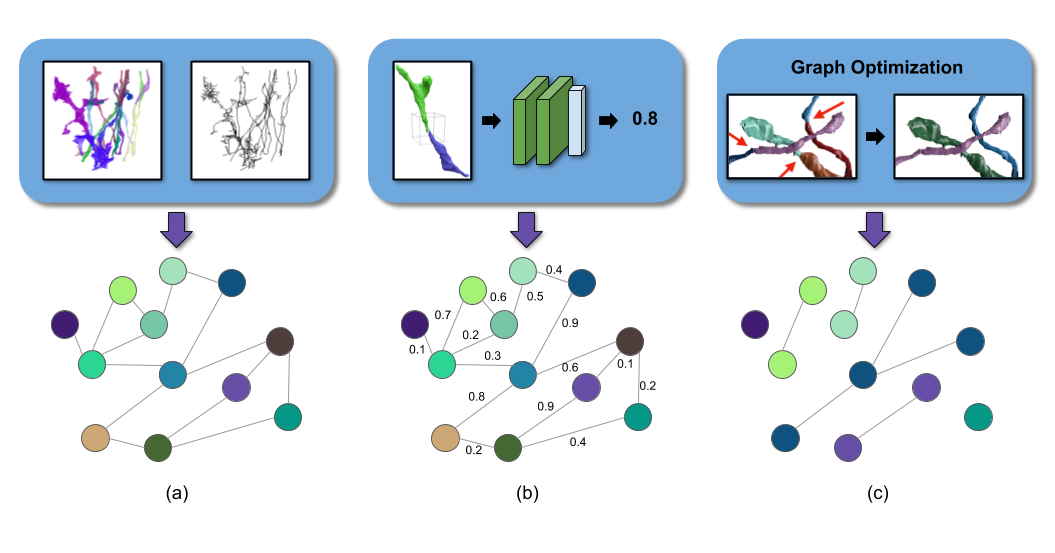
\includegraphics[width=0.75\linewidth]{./figures/teaser_v4.png}
	\caption{Our framework uses both geometric and topological biological constraints for region merging. We (a) generate a simplified graph from the skeleton representation of the input segmentation, (b) train a classifier to learn the edge weight based on the shape of the segment connection, and (c) perform graph partitioning with acyclic constraints.}
	\label{fig:teaser_pipeline}
\end{figure*}

A significant amount of connectomics research considers the problem of extracting segmentation information at the voxel level of EM images.
First, intermediate representations like boundary, affinity or binary segmentation maps are generated from the voxels.
Random forests with hand-designed features~\cite{kaynig2015large}, or 2D and 3D convolutional networks produce boundary probabilities~\cite{seymour2016rhoananet,ronneberger2015u,bogovic2013learned,ciresan2012deep,jain2010boundary,amelio_segmentation}.
Often, the affinity between each voxel and its six neighbors are used~\cite{lee2015recursive,parag2017anisotropic,lee2017superhuman,cciccek20163d,turaga2010convolutional}. 
The 3D U-Net architecture has become popular~\cite{cciccek20163d} and the MALIS cost function is specifically designed to re-weight affinity predictions by their contribution to the segmentation error~\cite{briggman2009maximin}.
More recently, flood-filling networks~\cite{januszewski2016flood} produce binary segmentations from raw pixels with a recurrent convolutional network at a high computational cost.
Orthogonal to the representation, model averaging~\cite{zeng2017deepem3d} and data augmentation~\cite{lee2017superhuman} methods can further improve the performance, where Lee et al.~\cite{lee2017superhuman} surpass the estimated human accuracy on the SNEMI3D dataset.

Clustering techniques transform these intermediate representations into segmentations.
Some early methods apply computationally expensive graph partitioning algorithms with a single node per superpixel~\cite{andres2012globally}.
Several pixel-based approaches generate probabilities that neighboring pixels belong to the same neuron.
Often a watershed algorithm will then cluster these pixels into super-pixels~\cite{zlateski2015image}.

Region merging methods can be categorized by the similarity metric between adjacent segments and the merging strategy.
For the similarity metric, Lee et al. and Funke et al. rely solely on the accuracy of the predicted affinities and define the metric as the mean affinity between segments~\cite{funke2017deep,lee2017superhuman}.
Classification-based methods generate the probability to merge two segments from handcrafted~\cite{jain2011learning,seymour2016rhoananet,nunez2014graph,10.1371/journal.pone.0125825,parag2017anisotropic,zlateski2015image} and learned features~\cite{bogovic2013learned}. 
For the merging strategy, most methods use variants of hierarchical agglomeration ~\cite{seymour2016rhoananet,nunez2014graph,10.1371/journal.pone.0125825,parag2017anisotropic,zlateski2015image} to greedily merge a pair of regions at a time.
Jain et al. formulates the agglomeration problem as a reinforcement learning problem ~\cite{jain2011learning} and Pape et al. present a scalable multicut algorithm to partition superpixels with global optimization~\cite{beier2017multicut}.

Additional research builds on top of these region-based methods to correct errors in the segmentation. This can be done either using human proofreading~\cite{haehn2017guided,haehn2014design,mojo2} or automatically~\cite{rolnick2017morphological,error_correction_using_CNN}. In both cases, available methods are pixel-based and do not include global biological constraints into the decision making process. Our method can be used as input to any existing error correction framework.

